\section{Storage Control}
\label{ch4:sec:storage-control}

In this section, the control of the energy storage system is explained.
More specifically, the Additive-Increase Multiplicative-Decrease (AIMD) algorithm is presented first, where its decision mechanism is explained in full.
Then the voltage referencing that is used for AIMD+ is detailed.

\subsection{AIMD algorithm}

\begin{algorithm}
\KwData{$p_\text{bat}(t)$, $\text{SOC}(t)$, $v_\text{bat}(t)$, $V_\text{thr}$, $V_\text{max}$, $V_\text{min}$, $\text{SOC}_\text{max}$, $\text{SOC}_\text{min}$, $\alpha$, $\beta$}
\KwResult{$p(t + \Delta t)$}
\For{$t\leftarrow 1$ \KwTo $T$}{
	 \tcp{Define the rate for the recent voltage reading}\label{cmt}
	 $r(t) = \left(v_\text{bat}(t) - V_\text{thr}\right)$\;
	 \eIf{$v_\text{bat}(t) \geq V_\text{thr}$}{
	 	\tcp{If voltage levels are above a threshold and...}\label{cmt}
	 	\eIf{$\text{SOC}(t) \leq \text{SOC}_\text{max}$}{
	 		\tcp{...SOC is not at max.: increase charging power}\label{cmt}
	 		$p(t + \Delta t) = p_\text{bat}(t) + \alpha P_\text{max}r(t)$
	 	}{
	 		\tcp{...SOC is at max.: shut off}\label{cmt}
	 		$p(t + \Delta t) = 0$\;
	 	}
	 	\tcp{If the battery has been discharging...}\label{cmt}
	 	\If{$p_\text{bat}(t) <0$}{
		 	\tcp{...reduce discharging power by $\beta$}\label{cmt}
		 	$p(t + \Delta t) = \beta p_\text{bat}(t)$\;
	 	}
	 }{
	 	\tcp{If voltage levels are below a threshold and...}\label{cmt}
	 	\eIf{$\text{SOC}(t) \geq \text{SOC}_\text{min}$}{
	 		\tcp{...SOC is not at min.: increase discharging power}\label{cmt}
	 		$p(t + \Delta t) = p_\text{bat}(t) - \alpha P_\text{max}r(t)$
	 	}{
	 		\tcp{...SOC is at min.: shut off}\label{cmt}
	 		$p(t + \Delta t) = 0$\;
	 	}
	 	\tcp{If the battery has been charging...}\label{cmt}
	 	\If{$p_\text{bat}(t) >0$}{
		 	\tcp{...reduce charging power by $\beta$}\label{cmt}
		 	$p(t + \Delta t) = \beta p_\text{bat}(t)$\;
	 	}
	 }
	 \tcp{Restrict power to BESS limits}\label{cmt}
	 $p_\text{bat}(t + \Delta t) = \textbf{signum}(p_\text{bat}(t)) \textbf{min}(|p_\text{bat}(t)|, P_\text{max})$\;
}
\caption{Compute battery power}
\label{ch4:alg:aimd}
\end{algorithm}


The proposed distributed battery storage control is shown in Algorithm~\ref{ch4:alg:aimd}.
This algorithm takes the current voltage reading, $v(t)$, current BESS power, $p(t)$, and the current state of charge, $\text{SOC}(t)$, as inputs and, with a set of control parameters, computes the next BESS power $p(t + \Delta t)$.
The two main parameters $\alpha$ and $\beta$, denotes the size of the power's additive increase step and the size of the multiplicative decrease step, respectively.
Therefore, $\alpha$ linearly increases and $\beta$ exponentially decreases, both charging and discharging powers (where discharging power is represented as a negative power flow since energy is released by the BESS).
The constants $V_\text{max}$ and $V_\text{thr}$ are the maximum historic voltage value and the set-point threshold used to regulate the total demand.
In the case when the total demand is too high, the local voltages will fall below $V_\text{thr}$, and the batteries reduce their charging power and start discharging.
This behaviour reduces total demand on the feeder.
At simulation start, $V_\text{max}$ is set to the nominal voltage of the substation transformer, i.e., 240 V, and $V_\text{thr}$ is set to a fraction of $V_\text{max}$, which was found by solving a balanced power flow analysis.
The variable $v(t)$ is the battery's local bus voltage, and $P_\text{max}$ denotes the maximum charging/discharging power of the battery.
The charging and discharging power of the batteries is increased in proportion to the available headroom on the network, which is inferred from the local voltage measurement $v(t)$, to avoid any sudden overloading of the substation transformer.

The algorithm itself, as shown in Algorithm~\ref{ch4:alg:aimd}, contains two decision levels.
The first determines whether the network is over- or under-loaded by comparing the local bus voltage, $v(t)$, to the battery's set-point threshold, $V_\text{thr}$ (line 4 and below).
In the event that the network is not under high load, the battery's SOC is compared to its operation limit to check whether the battery can charge, i.e., $\text{SOC}$ \textless $\text{SOC}_\text{max}$.
If there is enough charging capacity left, then the battery's charging power is linearly increased (line 6 and below).
If the battery was previously discharging, the related discharging power is exponentially reduced (line 14 and below) to reflect the multiplicative decrease.

The second decision level is entered when the network is under load (line 18 and below)
Here, the discharging power is linearly increased if the battery has enough energy stored, i.e. $\text{SOC}$ \textgreater $\text{SOC}_\text{min}$ (line 20 and below).
Additionally, if the battery was previously charging, then its charging power is multiplicatively reduced (line 28 and below).
The direction of the charging/discharging power adjustment is determined by the first decision level, as well as the threshold proximity ratio $r(t)$.
As the battery's bus voltage, $v(t)$, approaches the threshold voltage, $V_\text{thr}$, this ratio tends to zero and thus stops the battery operation.
Therefore, oscillatory hunting is effectively mitigated.
The last step of the algorithm (line 34) assures that the battery's charge/discharge power is within its device's ratings.

\subsection{Reference Voltage Profile}

When using a fixed voltage threshold, the difference in the location and load of each customer results in the over-utilisation of batteries located at the feeder end.
Similar to Papaioannou et al. \cite{Papaioannou2015}, yet for the control of BESS instead of EV charging, a reference voltage profile is proposed, which is produced by performing a power flow analysis of the network under maximum demand.
An example of a fixed threshold and reference voltage profile is shown in Figure~\ref{ch4:fig:ref-voltage-difference}.

In the AIMD+, consumers located at the head of the feeder are allocated a higher voltage threshold, while those towards the end of the feeder have similar voltage thresholds to that of the fixed threshold.
This replicates the expected voltage drop along the length of the feeder, hence resulting in a more equal utilisation of battery storage units that are located at those distances.
The voltage threshold is set in such a way as to limit the maximum voltage drop to 3\% at the end of the feeder.

\begin{figure}\centering
	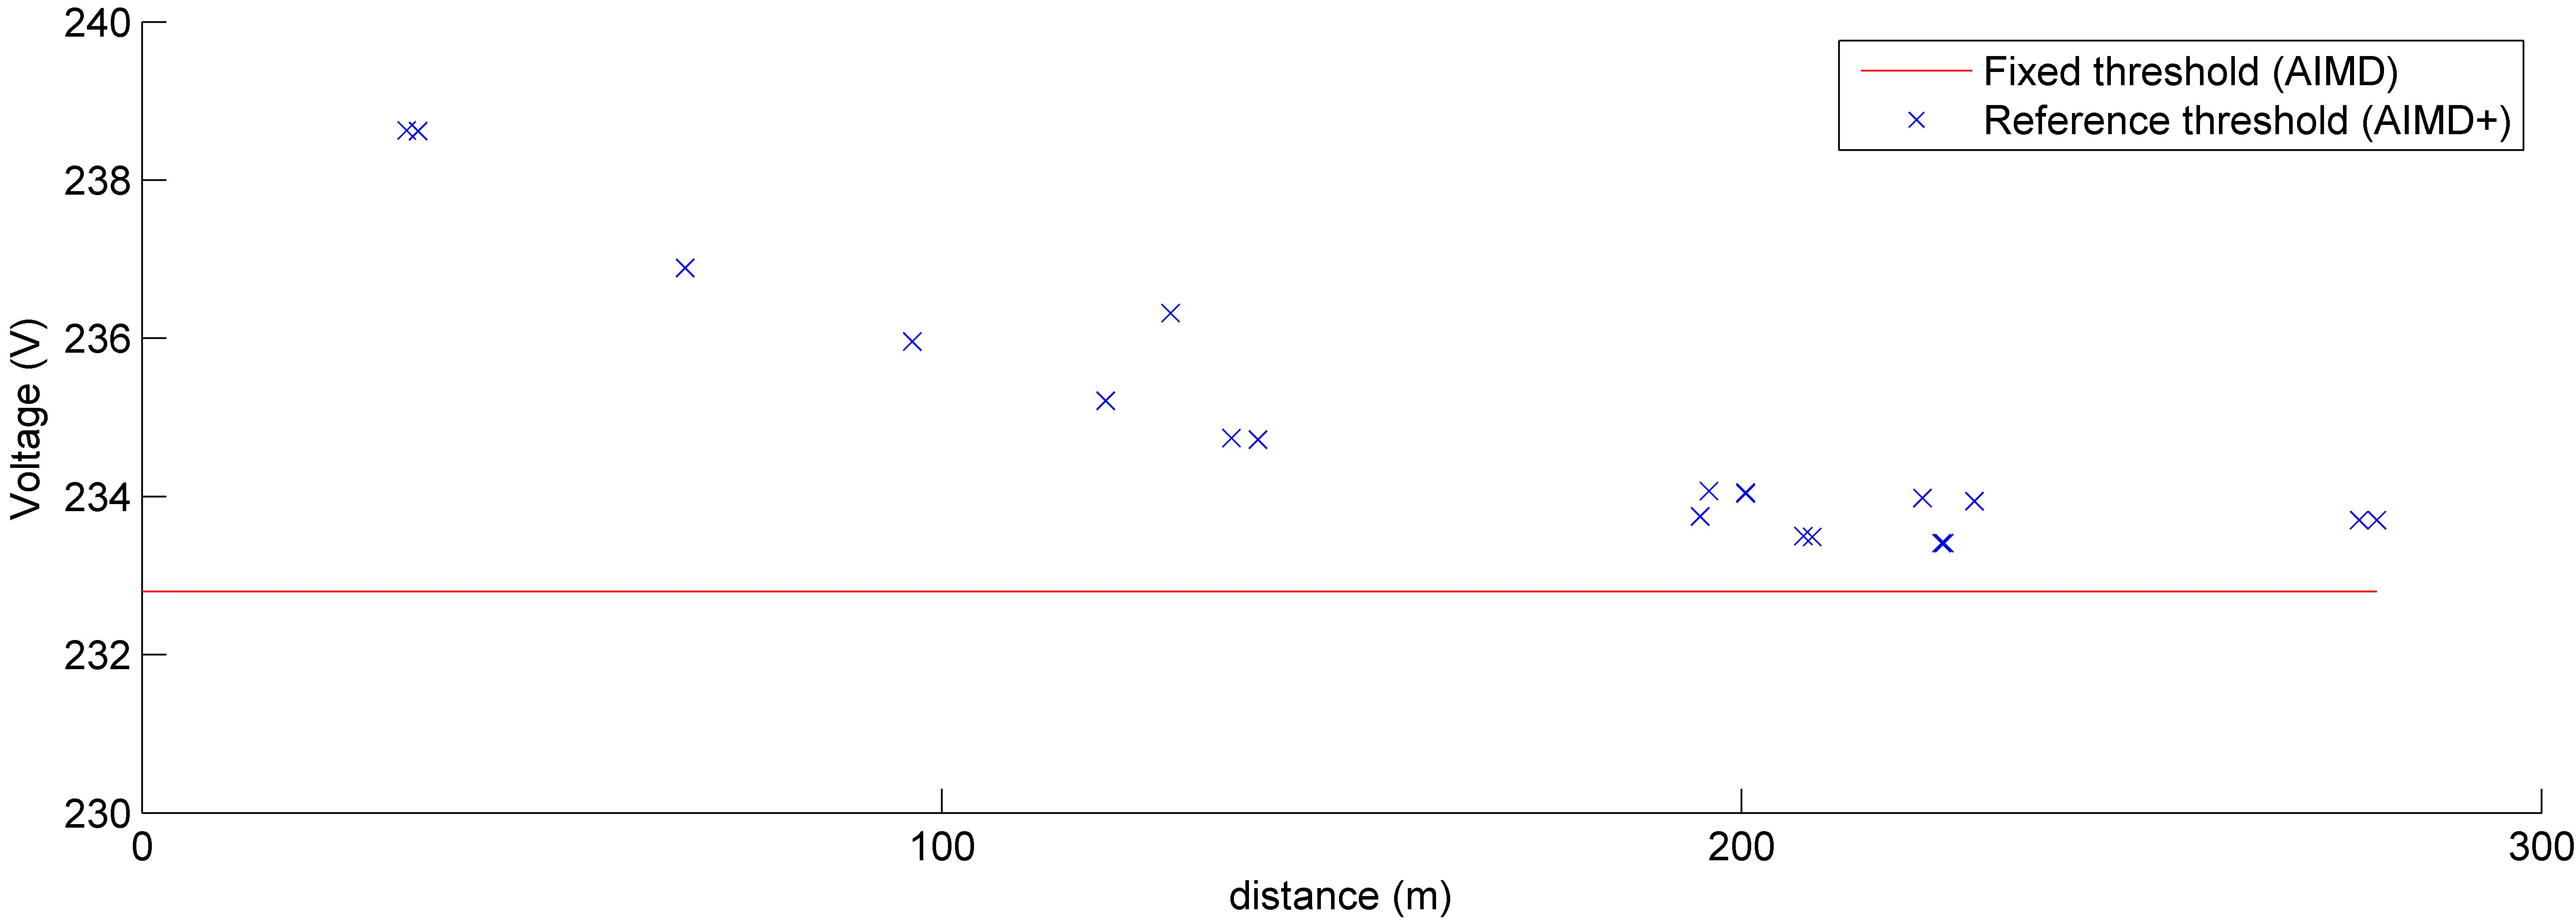
\includegraphics{_chapter4/fig/ref-voltage-difference}
	\caption{A plot showing the difference between the fixed voltage threshold (AIMD) and the reference voltage profile (AIMD+).}
	\label{ch4:fig:ref-voltage-difference}
\end{figure}

